\documentclass{article}


% if you need to pass options to natbib, use, e.g.:
\PassOptionsToPackage{numbers, sort&compress}{natbib}
% before loading neurips_2022


% ready for submission
\usepackage{neurips_2022}

% to compile a preprint version, e.g., for submission to arXiv, add add the
% [preprint] option:
%     \usepackage[preprint]{neurips_2022}


% to compile a camera-ready version, add the [final] option, e.g.:
%     \usepackage[final]{neurips_2022}


% to avoid loading the natbib package, add option nonatbib:
% \usepackage[nonatbib]{neurips_2022}


\usepackage[utf8]{inputenc} % allow utf-8 input
\usepackage[T1]{fontenc}    % use 8-bit T1 fonts
\usepackage{hyperref}
% \usepackage{subfigure}
\usepackage{graphicx}    % hyperlinks
\usepackage{url}            % simple URL typesetting
\usepackage{color}
\usepackage{booktabs}       % professional-quality tables
\usepackage{amsfonts}       % blackboard math symbols
\usepackage{nicefrac}       % compact symbols for 1/2, etc.
\usepackage{microtype}      % microtypography
\usepackage{xcolor}         % colors
\usepackage{wrapfig}


\usepackage{times}
\usepackage{epsfig}
\usepackage{amsmath}
\usepackage{amssymb}

% Include other packages here, before hyperref.
\usepackage{float}
\usepackage{bbding}
\usepackage{pifont}
\usepackage{wasysym}
\usepackage{multirow}
\usepackage{subfig}



\title{Self-Supervised Spatial Temporal Feature Learning for Video Correspondence}


% The \author macro works with any number of authors. There are two commands
% used to separate the names and addresses of multiple authors: \And and \AND.
%
% Using \And between authors leaves it to LaTeX to determine where to break the
% lines. Using \AND forces a line break at that point. So, if LaTeX puts 3 of 4
% authors names on the first line, and the last on the second line, try using
% \AND instead of \And before the third author name.

\author{%
  David S.~Hippocampus\thanks{Use footnote for providing further information
    about author (webpage, alternative address)---\emph{not} for acknowledging
    funding agencies.} \\
  Department of Computer Science\\
  Cranberry-Lemon University\\
  Pittsburgh, PA 15213 \\
  \texttt{hippo@cs.cranberry-lemon.edu} \\
  % examples of more authors
  % \And
  % Coauthor \\
  % Affiliation \\
  % Address \\
  % \texttt{email} \\
  % \AND
  % Coauthor \\
  % Affiliation \\
  % Address \\
  % \texttt{email} \\
  % \And
  % Coauthor \\
  % Affiliation \\
  % Address \\
  % \texttt{email} \\
  % \And
  % Coauthor \\
  % Affiliation \\
  % Address \\
  % \texttt{email} \\
}


\begin{document}


\maketitle


\begin{abstract}
  This paper proposes to learn reliable dense correspondence from videos in a self-supervised manner. Our learning process integrates two highly related tasks: tracking large image regions and establishing fine-grained pixel-level associations between consecutive video frames. We exploit the synergy between both tasks through a shared inter-frame affinity matrix, which simultaneously models transitions between video frames at both the region- and pixel-levels. While region-level localization helps reduce ambiguities in fine-grained matching by narrowing down search regions; fine-grained matching provides bottom-up features to facilitate region-level localization. Our method outperforms the state-of-the-art self-supervised methods on a variety of visual correspondence tasks, including video-object and part-segmentation propagation, keypoint tracking, and object tracking. Our self-supervised method even surpasses the fully-supervised affinity feature representation obtained from a ResNet-18 pre-trained on the ImageNet.
\end{abstract}



\section{Introduction}
Learning representations for video correspondence is a fundamental problem in computer vision, which is closely related to different video applications, including optical flow estimation~\cite{dosovitskiy2015flownet}\cite{horn1981determining}, video object segmentation~\cite{caelles2017one}\cite{oh2019video}, keypoint tracking~\cite{xiu2018pose}, etc. However, supervising such a representation requires a large number of dense annotations, which is unaffordable. Thus most approaches acquire supervision from simulations or limited annotations, which result in poor generalization in different downstream tasks. Recently, self-supervised feature learning is gaining significant momentum, and several pretext tasks are designed for space-time visual correspondence using abundant unlabeled videos. 

The key to this task lies in two different perspectives. The first one is \textbf{temporal feature learning}, which aims to learn the fine-grained correspondence of pixel/object between frames. With the nature of temporal coherence in the video, the temporal feature learning can be formed as a reconstruction task, where the query pixel in the target frame can be reconstructed by leveraging the information of adjacent reference frames within a local region. Then a reconstruction loss is applied to minimize the photometric error between the raw frame and its reconstruction. However, in real videos, the temporal discontinuity occurs frequently due to the occlusions, dramatic appearance changes, and deformations, especially for pixels in each frame with severe down-sampling. In such scenarios, the frame reconstruction loss apparently becomes invalid, which result in inferior performance. MAST~\cite{lai2020mast} proposes to apply frame reconstruction with a higher feature resolution by decreasing the stride of the backbone, which requires a larger memory and computation cost. Besides, the frame reconstruction is achieved under the assumption of temporal continuity, thus fail to learn representation that is invariant to appearance change in time.  Another way to exploit the free temporal supervision is by exploiting temporal cycle-consistency.  \cite{jabri2020space}\cite{wang2019learning} track object forward and backward with the objective of maximizing the temporal cycle correspondence consistency with reconstruction and contrastive loss. However, compared to the correspondence which is realized at object-level, the frame reconstruction is conducted on raw image space, which provides more accurate supervision for learning fine-grained correspondence.

\begin{figure}[!tb]
  \centering
  {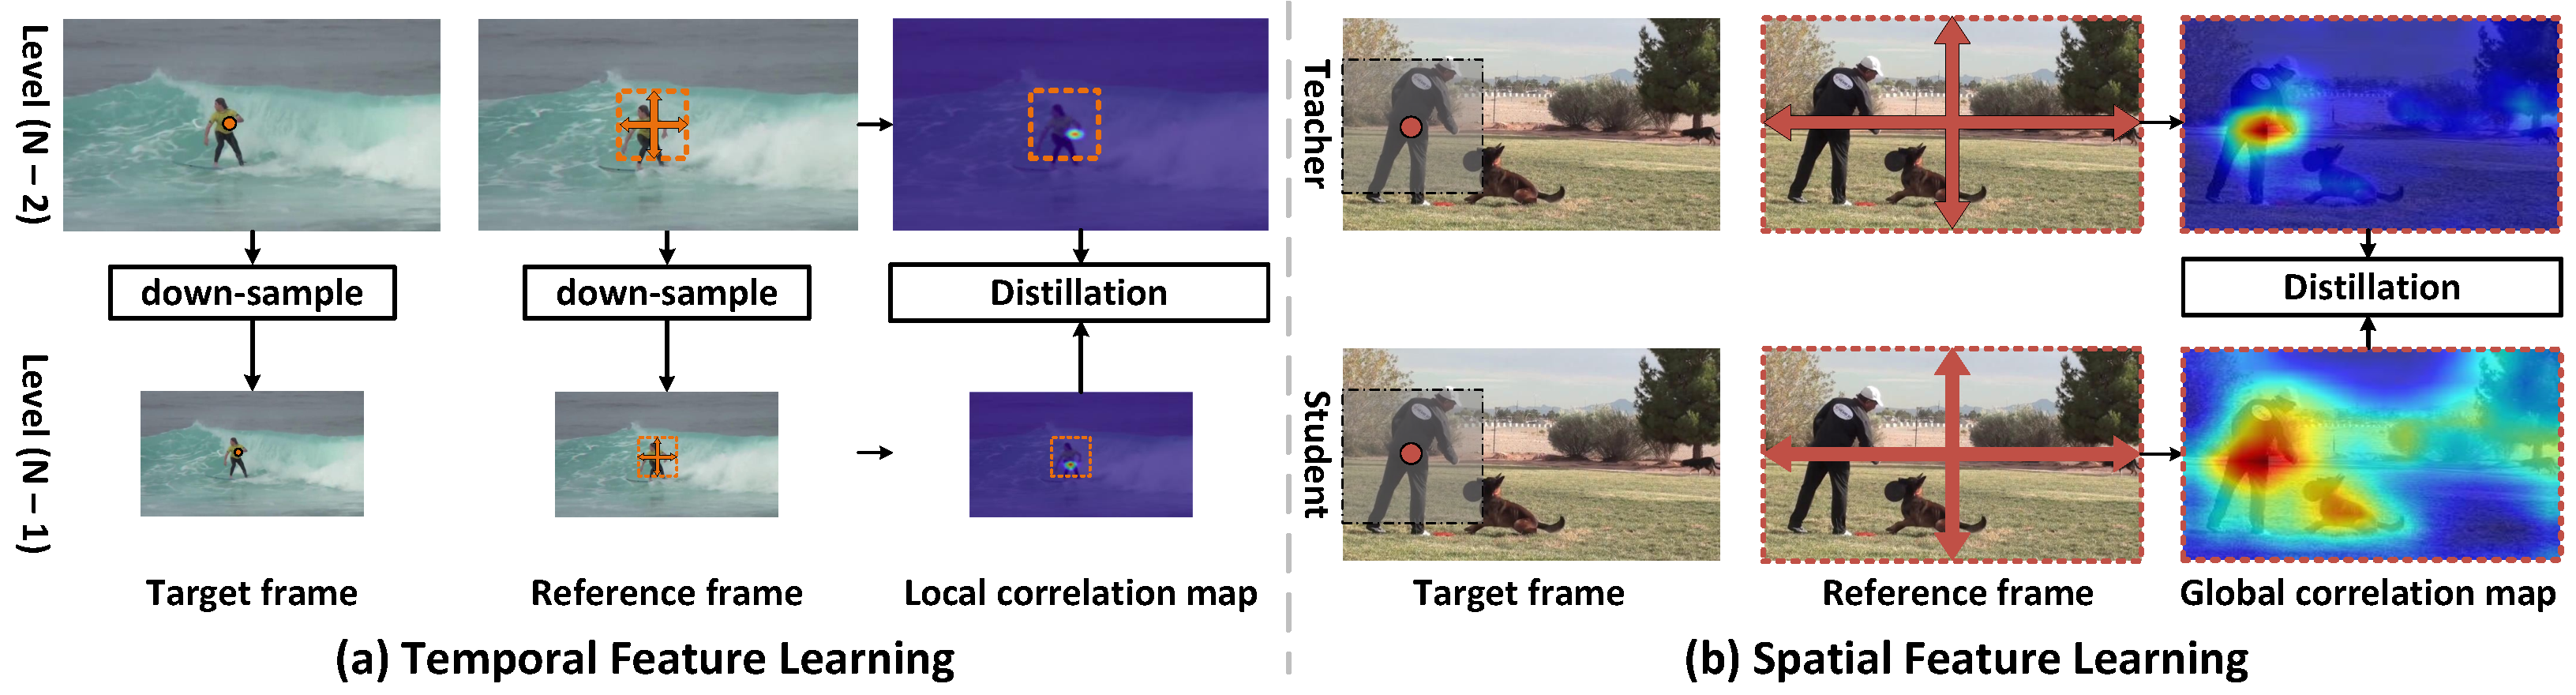
\includegraphics[width=1.0\textwidth]{figure/tissor/tissor6.pdf}}
  \caption{\small Visualization of our key idea. Given a query point randomly sampled in target frame, we visualize the result of computing the local correlation and global correlation map $w.r.t.$ reference frame. The dashed line in red represents the range of computing correlation map $w.r.t.$ query point. The reference frame is randomly sampled in the memory bank of inference strategy [11]. }
  \label{fig:tissor}
  \vspace{-6mm}
\end{figure}

The second one is \textbf{spatial feature learning}, which pays more attention to learning the object appearance that is invariant to viewpoint and deformation changes. \cite{wang2020contrastive} adopts a novel intra-inter consistency loss to learn inter-video discriminative feature while \cite{xu2021rethinking} learns the space-time correspondence through a frame-wise contrastive loss. However, both methods are trained on video datasets and try to realize the spatial and temporal feature learning in a unified framework, which is sub-optimal for each of them. Recently, as mentioned in~\cite{wang2021different}, the contrastive model~\cite{he2020momentum}\cite{xie2021detco} pre-trained on image data shows impressive performance for video correspondence. This motivates us to design a framework that learns the spatial and temporal feature independently with image and video data.  

In this paper, we decouple video correspondence learning into two separate processes, including spatial and temporal feature learning. To achieve this, we first train the model in a contrastive learning paradigm on ImageNet~\cite{deng2009large}, which gives the model the ability to capture object appearance. Then, instead of training with a large video dataset, $i.e.$, Kinetics~\cite{carreira2017quo} with 300k videos, we perform the temporal feature learning on YouTube-VOS~\cite{xu2018youtube}, which consists of 3.5k videos. However, apart from the severe  information lost and temporal discontinuity due to large spatial down-sampling on frames, directly fine-tuning the old model with only new data will leads to a well-known phenomenon of catastrophic forgetting~\cite{li2017learning}. To address the first problem, we propose a novel pyramid learning framework. The frame reconstruction is applied at different levels of network to better exploit the free temporal supervision. As you can see in Figure \ref{fig:tissor} (a), the pixels of target and reference frame with higher resolution have a lower chance of occurring temporal discontinuity, which provides a more accurate local correlation map. Thus we design a new loss named \textbf{local correlation distillation loss} that supports explicitly learning of the correlation map in the region with high uncertainty, which is achieved by taking the finest local correlation map as pseudo labels. At the same time, as shown in Figure \ref{fig:tissor} (b), we freeze the model pre-trained on ImageNet as teacher. Then a \textbf{global correlation distillation loss} is proposed to keep the student the ability of capturing object-level correspondence which is closely related to object appearance modeling. 

To sum up, our main contributions include: (a) We propose a decoupled learning paradigm for self-supervised video correspondence, including spatial and temporal feature learning. (b) We propose a pyramid learning framework with local correlation distillation to enable the model to estimate fine-grained correspondence. (c) We introduce a global correlation distillation loss to keep the ability of capturing object appearance when training on video dataset. (d) Last but not least, we verify the proposed approach in a series of correspondence-related tasks including video object segmentation, human parts propagation and pose tracking. Our approach consistently outperforms previous state-of-the-art self-supervised methods and is even comparable with some task-specific fully-supervised algorithms.

\section{Related Work}
\textbf{Self-supervised learning for video correspondence.} 
Recent approaches focus on learning correspondence from unlabeled videos in a self-supervised manner. The task requires the model to have the ability to capture object appearance and estimate the fine-grained correspondence between frames at the same time, which has proceeded along two different dimensions: reconstruction-based methods and cycle-consistency-based methods. In the first type, a query point is reconstructed from adjacent frames while the latter performs forward-backward tracking with the objective of minimize the cycle inconsistency. Through getting promising results, most methods address the problem considering only one perspective. VFS learns the spatial temporal representation through a frame-wise contrastive loss while DUL and Contra try to realize the spatial and temporal feature learning in a unified framework by exploiting the inter-video constraint, which may result in sub-optimal performance. In this paper, we learn a better representation by decoupling the video correspondence learning to two separate processes including spatial and temporal feature learning.


\textbf{Self-supervised spatial feature learning.} Self-supervised spatial feature learning aims to learn discriminative feature of object appearance with unlabeled data, which recently has get promising result with contrastive learning. In an early work [44], the constrastive learning is formulated as instance discrimination task, which requires the model to return low values for similar pairs and high values for dissimilar pairs. Recently, the performance is further improved by creating a dynamic memory-bank, introducing online clustering and avoiding the use of negative pairs. Further more, DensCL, InsLoc and DetCo propose various pre-text tasks to adapt the contrastive learning to tasks which require dense prediction. Even through showing superior performance for video correspondence learning~[11], the contrastive model pre-trained on image data still struggles to modeling the fine-graied correspondence between video frames. 

\textbf{Self-supervised temporal feature learning. } 
Compared to spatial feature learning, temporal feature learning focus on learning the motion information of video, which is closely related to optical flow and motion estimation. Most methods [12][11] directly regress the groundtruth optical flow produced by synthetic datasets thus suffering from severe domain shift. To deal with the problem, [1][3] try to learn the dense correspondence on real video without any label by minimizing the photometric error between the raw frame and its reconstruction. However, the video frames usually contain temporal discontinuity including dramatic appearance change and occlusions, which seriously degrades the capability of the method. [12][14] alleviate the problem by utilizing the optical flow predictions from teacher model to guide the learning of student model in the region with occlusions. In this paper, we address the issue from two perspectives: (1)~Learning a better representation that is invariant for appearance change. (2)~Supervising the correlation by taking the finest corelation as pseudo labels.


\begin{figure}[!tb]
  \centering
  {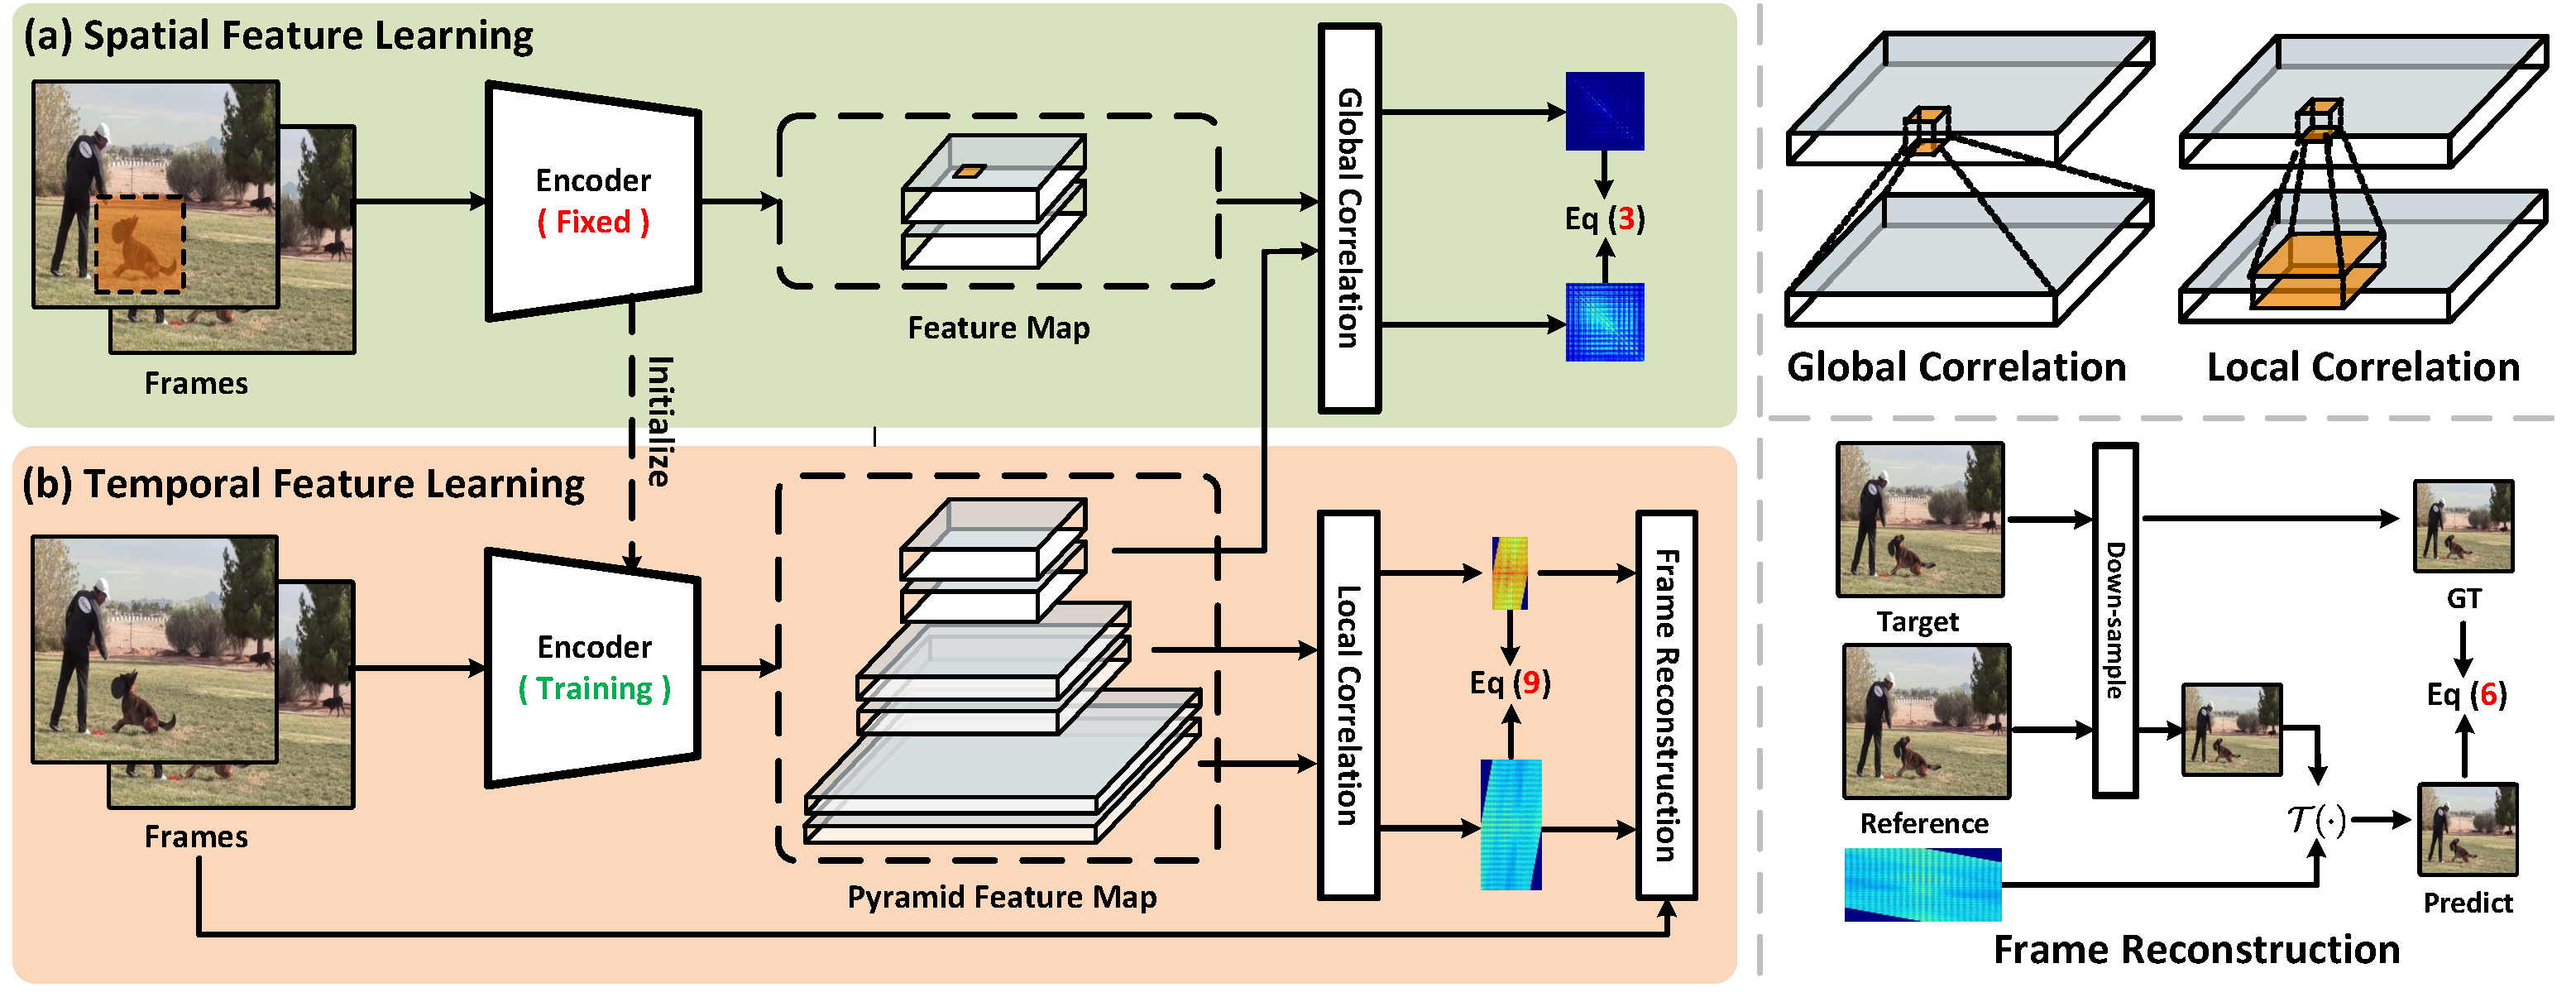
\includegraphics[width=1.0\textwidth]{figure/framework/framework.pdf}}
  \caption{\small An overview of our spatial temporal feature learning framework. Our method  decouples video correspondence learning into two separate processes including spatial feature learning and temporal feature learning. Specifically, the \textbf{spatial feature learning} first exploits the contrastive loss which is analogous to that of instance discrimination to learn the object appearance with image data. Then we perform the self-supervised training with video data in the next step. To maintain the ability to capture object appearance, we fix the pre-trained network as teacher and a global correlation distillation is devised.  For \textbf{temporal feature learning}, we propose a pyramid learning framework where the frame reconstruction is devised at each levels of network. As the same time, we introduce a novel loss named local correlation distillation loss that supports explicitly learning of the correlation map at the region with high uncertainty, which is achieved by taking the finest local correlation map as pseudo labels.}
  \label{fig:framework}
  \vspace{-7mm}
\end{figure}



\section{Approach}
The basic idea of our method is to decouple video correspondence learning into two separate processes including spatial feature learning and temporal feature learning. We first train our model using contrastive loss with image data to learn the object appearance that is invariant to viewpoint. Then, we perform the temporal feature learning on a small video dataset to learn the fine-grained correspondence between frames. To deal with the problems including temporal discontinuity and catastrophic forgetting when training on video data, a pyramid learning framework is proposed with local and global correlation distillation loss.

\subsection{Spatial Feature Learning}
\label{spatial_feature_learning}
The spatial feature mainly describes appearance of objects involved in a image. Spatial feature learning is analogous to that of instance discrimination, and thus easily benefits from the recent advancements brought by contrastive learning. We firstly briefly reviewing instance discrimination objective in contrastive learning. Given an encoded query $\boldsymbol{q}\in\mathbb{R}^d$ and a set of encoded key vectors $\mathcal{K}=\left\{\boldsymbol{k}^{+}, \boldsymbol{k}_{1}^{-}, \boldsymbol{k}_{2}^{-}, \ldots, \boldsymbol{k}_{K}^{-}\right\}$ which consists of one positive key $\boldsymbol{k}^{+}\in\mathbb{R}^d$ and $K$ negative keys $\mathcal{K^{-}}=\left\{\boldsymbol{k}_{j}^{-}\right\}$, where $d$ denotes the embedding dimension. The query and its positive key are generated from  same instance with two different augmentations, while the negative keys ref to other instances. The objective of instance discrimination is to maximize the similarity between the query $\boldsymbol{q}$ and the positive key $\boldsymbol{k}^{+}$ while remains query distinct to all negative keys $\mathcal{K^{-}}$. Thus, a contrastive loss is presented in InfoNCE  with a softmax formulation:
	\begin{equation}\label{eq:nce}
		\small
		\begin{aligned}
			\mathcal{L}_{\text{nce}}=-\log \frac{\exp \left(\boldsymbol{q}^{T} \boldsymbol{k}^{+} / \tau_c\right)}{\exp \left(\boldsymbol{q}^{T} \boldsymbol{k}^{+} / \tau_c\right)+\sum_{i=1}^{K} \exp \left(\boldsymbol{q}^{T} \boldsymbol{k}_{i}^{-} / \tau_c\right)}
		\end{aligned}~~,
	\end{equation}
	where the similarity is measured via dot product, and $\tau_c$ is the temperature hyper-parameter. MoCo [14] builds a dynamic memory bank to maintain a large number of negative samples with a moving-averaged encoder. DetCo [15] further improves the contrastive loss $\mathcal{L}_{\text{nce}}$ by introducing a global and local contrastive learning to enhance local representation for dense prediction. In this paper, we adopt the same framework as MoCo [14] and DetCo [15] to learn a appearance model for most of our experiments.\\
\\
\textbf{Global correlation distillation.} After main training with contrastive loss, we get a encoder $\phi$. Then we continuously train it on video data to learn the fine-grained correspondence ( See section \ref{temporal_feature_learning} ). However, directly fine-tuning the old model with only new data will lead to a well-known phenomenon of catastrophic forgetting, which degrades the performance. Thus we introduce a global correlation distillation loss in order to maintain the ability to capture object appearance. More specifically, we first fix the feature encoder $\phi$ as teacher denoted as $\phi_t$. Given a pair of video frames consisting of target and reference frame $I_{t}, I_r \in \mathbb{R}^{H\times W \times 3}$, the  $\phi$ maps them to a pair of feature embeddings $F^l_t,F^l_{r} \in \mathbb{R}^{h^l\times w^l \times d^l}$, where $l \in \{0, 1, \ldots, N \}$ is the index of each pyramid level and the smaller number represents the coarser level. Here $l$ is set to $N$. For each query point $F^l_t(i)$ and key point $F^l_r(j)$, we have global correlation $a_{i, j}$ ( See Figure \ref{fig:framework} ) using a softmax over similarities $w. r. t.$ all keys in reference frame, $i. e$:\\
\begin{equation}\label{eq:global_correlation}
  \small
  \begin{aligned}
    a_{i, j}=\frac{\exp \left(F^l_t(i)  \cdot F^l_r(j) / \tau\right)}{\sum_{n} \exp \left(F^l_t(i) \cdot F^l_r(n) / \tau\right)}, i,j,n \in \{1,\ldots,h^lw^l\}
  \end{aligned}~~,
\end{equation}
Where ‘·’ stands for the dot product. Each point in $F^l_t$ and $F^l_{r}$ covers a relatively large region \textcolor{red}{since the output stride is set to 32 in our feature encoder.} Thus we can form the correlation as object-level correspondence which is closely related to object appearance. We generate the pseudo labels of global correlation distillation by computing the global correlation  $a^t_{i, j}$ for each query with teacher $\phi_t$. The global correlation distillation loss is defined to minimize the mean squared error between $a$ and $a^t$:\\
\begin{equation}\label{eq:global_correlation_loss}
  \small
  \begin{aligned}
    % \mathcal{L}_{gc}  =\sum_{i}\sum_{j} \left\|a_{i,j}-a^t_{i,j}\right\|_{2}^{2}
    \mathcal{L}_{\mathrm{gc}}  = \left\|a-a^t\right\|_{2}^{2}
  \end{aligned}~~,
\end{equation}

\subsection{Temporal Feature Learning}
\label{temporal_feature_learning}
We then perform temporal feature learning right after spatial feature learning. Temporal feature learning aims to learn the fine-grained correspondence between video frames. Recently, a few studies [40, 84] introduce a reconstruction-based correspondence learning scheme, where each query pixel in the target frame can be reconstructed by leveraging the information of adjacent reference frames within a local region. More specifically, the target and reference frame $I_{t}, I_r$ are projected into a  fine-grained pixel embedding space. We denoted these embedding as $F_t,F_{r} \in \mathbb{R}^{hw \times d}$. For each query pixel $i$ in $I_{t}$, we can calculate the local correlation $c_{i,j}$ with reference frame within a local region with a softmax formulation:
\begin{equation}\label{eq:local_correlation}
  \small
  \begin{aligned}
    c_{i, j}=\frac{\exp \left(F_t(i)  \cdot F_r(j) / \tau\right)}{\sum_{n} \exp \left(F_t(i) \cdot F_r(n) / \tau\right)}, i \in \{1,\ldots,hw\}, j,n \in \mathcal{N}(i)
  \end{aligned}~~,
\end{equation}
Where $\mathcal{N}(i)$ is the index set with a limited range of $r$ pixels for pixel $i$ ( see Figure \ref{fig:framework} ). Then each query pixel $i$ in target frame can be reconstructed by a weighted-sum of pixels in $\mathcal{N}(i)$, according the local correlation map $c \in \mathbb{R}^{hw \times (r)^2}$:
\begin{equation}\label{eq:reconstruction}
  \small
  \begin{aligned}
    \hat{I}_{t}(i)=\sum_{j \in \mathcal{N}(i)} c_{i,j} I_{r}(j)
  \end{aligned}~~,
\end{equation}
We regard the above process as a transformation function for all query pixels and denotes it as: $\hat{I}_{t} = \mathcal{T}\left(c, I_t\right)$. Then the reconstruction loss is defined as L1 distance between $\hat{I}_{t}$ and $I_{t}$:
\begin{equation}\label{eq:reconstruction loss}
  \small
  \begin{aligned}
    \mathcal{L}_{\mathrm{rec}}=\left\|I_{t}-\hat{I}_{t}\right\|_{1}
  \end{aligned}~~,
\end{equation}
However, the Eq \ref{eq:reconstruction} should only be applied when the feature embedding has same size with video frame. Thus the stride of $\phi$ must be set to 1, which introduces large memory and computation cost. One possible solution is to apply down-sampling on target frame. MAST propose a image feature alignment module which sampling the pixel at center of strided convolution kernels. However, down-sampling with large rate would not only cause severe information lost of supervision but also result in more pixel occlusions between video frames, which obviously degrades the representation of temporal feature learning. To alleviate the problem, we design a pyramid learning framework consisting of pyramid frame reconstruction and local correlation distillation with entropy-based selection.\\
\\
\textbf{Pyramid frame reconstruction.}  As you can see in Figure \ref{fig:framework}, we obtain a pair of feature pyramids $\{F^l_t\}^{N-1}_{l=1}$,$\{F^l_{r}\}^{N-1}_{l=1}$.  Then we get the pyramid local corelation map $\{c^l\}^{N-1}_{l=1}$ at each level by utilizing Eq \ref{eq:local_correlation} with different local range $r^l$. As the same time, we adopt a same down-sampling method as [1] to obtain a pair of frame pyramids $\{I^l_t\}^{N-1}_{l=1},\{I^l_{r}\}^{N-1}_{l=1}$, which has same shape with the feature pyramids at each level. Given the $c^l$, $I^l_t$ and $I^l_r$, we apply the pyramid reconstruction loss at each level:
\begin{equation}\label{eq:pyramid reconstruction loss}
  \small
  \begin{aligned}
    \mathcal{L}^{p}_{\mathrm{rec}}=\sum_l\left\|I^l_{t}-\mathcal{T}\left(c^l, I^l_r\right)\right\|_{1}
  \end{aligned}~~,
\end{equation}
By doing this, we are able to exploit more free temporal supervision and get better temporal representation at intermediate level. \\
\\
\textbf{Local correlation distillation.} The bottom level of the frame pyramid contains more rich information and serfer less occlusions for temporal feature learning due to relatively small down-sampling rate, which may result in more accurate local correlation map. Inspired by it, we design a novel local correlation distillation loss which explicitly make constraint on the final local correlation map $c^{N-1} \in \mathbb{R}^{h^{N-1}w^{N-1} \times (r^{N-1})^2}$. We first compute the local correlation map $c^{N-2}$ at level $N-2$ and then apply  correlation down-sampling [16] to get pseudo labels $c^t$ with the same size as $c^{N-1}$.  Then the local correlation distillation loss $\mathcal{L}_{lc}$ is adopt to minimize the mean squared error between $c^{N-1}$ and $c^t$.\\

\textbf{Entropy-based selection.} The correlation of each query $w.r.t$ reference frame indicates more uncertainty when having smooth distribution, which should be paid more attention when applying distillation. Thus we calculate the entropy for each query $i$:
\begin{equation}\label{eq:pyramid reconstruction loss}
  \small
  \begin{aligned}
    \mathcal{H}(i)=\sum_j-log c^{N-1}_{i,j}
  \end{aligned}~~,
\end{equation}
Then we obtain a mask $m \in \mathbb{R}^{h^{N-1}w^{N-1}}$ to filter out the region with lower entropy by setting a threshold $T$. The local correlation distillation loss with entropy selection is defined as:
\begin{equation}\label{eq:reconstruction loss}
  \small
  \begin{aligned}
    \mathcal{L}^e_{\mathrm{lc}}=\sum_im_i\left\|c_{i,:}^{N-1}-c_{i,:}^t\right\|^2_{2}
  \end{aligned}~~,
\end{equation}
Eventually, our training loss of temporal feature learning is defined as: $\mathcal{L}_\mathrm{t}$ =  $\mathcal{L}^p_{\mathrm{rec}} + \alpha  \mathcal{L}^e_{\mathrm{lc}}$. The final loss of training on video data is a weighted sum of  $\mathcal{L}_\mathrm{t}$ and a regularization term $\mathcal{L}_\mathrm{gc}$ introduced in Section \ref{spatial_feature_learning}:
\begin{equation}\label{eq:final loss}
  \small
  \begin{aligned}
    \mathcal{L} = \mathcal{L}_{\mathrm{t}}  + \beta  \mathcal{L}_{\mathrm{gc}}
  \end{aligned}~~,
\end{equation}


\section{Experiments}
We verify the merit of our method in a series of correspondence-related tasks, including semi-supervised video object segmentation, pose keypoints tracking, human parts segmentation propagation. In this section we will first introduce our experiments settings including details of implementation  and evaluation. Then detailed ablation studies are performed to  explain how each component of our method works. Last but not least, we finally report the performance comparision with state-of-the-art methods to further verify the effectiveness of our method.
\subsection{Implementation Details}
\textbf{Architectures.} We exploit the encoder $\phi$ with both ResNet-18 and ResNet-50 [27, 37] for self-supervised training. Following prior works [12], we reduce the stride of convolutional layers in $\phi$ to increase the spatial resolution of feature maps on layer $res4$  by a factor of 4 or 8 ($i.e,$ downsampling rate 8 or 4). 
Further more we set the stride of $res5$ layer to 4 in order to increase the receptive filed for spatial feature learning.

\textbf{Training.}
We first train our model using contrastive loss for 200 epochs on ImageNet following most hyper-parameters settings of [76]. Then we perform temporal feature learning on YouTube-VOS train set [16] which consists of 3.5k videos. In this stage, the video frame is resized into 256$\times$256 and channel-wise dropout in Lab color space [39] is adopted as the information bottleneck. We train the encoder for 100k iterations with mini-batch of 128  using Adam as our optimizer. The initial learning rate is set to 1e-4 with a cosine (half-period) learning rate schedule. The frame reconstruction is applied on both $res3$ and $res4$ layer while we realize global correlation distillation on $res5$ layer.

\textbf{Evaluation.}
We follow the same evaluation protocol and downstream tasks in [33, 71]. We directly utilize unsupervised pre-trained model as the feature extractor without any fine-tuning.  Given the input frame with  spatial resolution of $H\times W$, the evaluation is realized on the $res4$ layer with a spatial resolution of $\frac{H}{8} \times \frac{W}{8}$ or $\frac{H}{4} \times \frac{W}{4}$. To propagate the semantic labels from the initial ground-truth annotation, the recurrent inference strategy is applied following recent works [12]. More specifically,  the semantical label of first frame as well as previous predictions are propagated to the current frame with the help of affinity between video frames. We evaluate our method over three downstream tasks including semi-supervised video object segmentation in DAVIS-2017 [8], human part propagation in VIP [10] and human pose tracking in JHMDB [9].

\subsection{Ablation Study}
The ablation study is performed with semi-supervised video object segmentation on DAVIS-2017 validation set. Following the official protocol [68], we use the mean of region similarity $\mathcal{J}_m$, mean of contour accuracy $\mathcal{F}_m$ and their average $\mathcal{J} \& \mathcal{F}_m$ as the evaluation metrics. We conduct a series of experiments to prove the effectiveness of each  component. The stride of encoder is all set to 8 for training and evaluation.

\begin{table*}[t]
  \centering
	\vspace{-1.5em}
    \hspace{0.1em}
    \small
    \renewcommand\thetable{5}
            \subfloat[{Ablation study of each component.} \label{table:ablation2}]{
              \resizebox{0.6\textwidth}{!}{
              %   \tablestyle{1pt}{1.1}
            \begin{tabular}{c|cc|cccc|ccc}
              \hline
              \# &
              $\mathcal{L}_{\mathrm{nce}}$ &
              $\mathcal{L}_{\mathrm{gc}}$ &
              $\mathcal{L}_{\mathrm{rec}}$ &
              % $\mathcal{L}^{p}_{\mathrm{rec}}$ &
              $p$ &
              $\mathcal{L}_{\mathrm{lc}}$ &
              % $\mathcal{L}^e_{\mathrm{lc}}$ &
              $e$ &
              Dataset &
              Arch &
                $\mathcal{J} \& \mathcal{F}_m \uparrow$ \\ 
              \hline
              % 1&$\checkmark$& & &             &   &   & I&Res18&61.7 \\
              % \hline
              1&&&$\checkmark$ & &  &   &    YTV& Res18 &64.6 \\
              2&&& $\checkmark$ & $\checkmark$&  &  &    YTV& Res18 &65.4 \\
              3&&& $\checkmark$& $\checkmark$& $\checkmark$ &   &    YTV& Res18 &68.1 \\
              4&&& $\checkmark$& $\checkmark$& $\checkmark$ &  $\checkmark$ &   YTV& Res18 & 69.0 \\ 
              \hline
              5&$\checkmark$& &$\checkmark$& $\checkmark$& $\checkmark$ &  $\checkmark$ &   I + YTV & Res18 & 69.3 \\ 
              6&$\checkmark$& $\checkmark$  &$\checkmark$& $\checkmark$& $\checkmark$ &  $\checkmark$ &   I + YTV & Res18 & \textbf{70.5} \\ 
              \hline
            \end{tabular}%
              }
            }
            \subfloat[{Ablation study of $\mathcal{L}_{\mathrm{gc}}$.} \label{table:ablation2}]{
            \resizebox{0.38\textwidth}{!}{
            % \tablestyle{1pt}{1.1}
            \begin{tabular}{@{}cccc@{}}
            \hline
            Method         & Dataset       & Arch &$\mathcal{J} \& \mathcal{F}_m \uparrow$ \\ 
            \hline
            $\mathcal{L}_{\mathrm{nce}}$ & I         & Res50 &66.5          \\
            w $\mathcal{L}_{\mathrm{t}}$    & I + YTV & Res50 &69.6          \\
            % + EWC            & ImageNet & Res50 &68.9          \\
            w $\mathcal{L}_{\mathrm{t}}$ + LwF            & I + YTV & Res50 &69.9          \\
            w $\mathcal{L}_{\mathrm{t}}$ + $\mathcal{L}_{\mathrm{gc}}$ & I + YTV & Res50 &\textbf{71.3} \\ 
            \hline
            \end{tabular}%
            }
          }
    \captionsetup{font=small}
    \caption{Ablation study for each component in spatial and temporal feature learning.  The "$p$" and "$e$" in (a) correspond to pyramid frame reconstruction and entropy-based selection. Models in (b) are all pre-trained on ImageNet with contrastive loss and models with "w" are subsequently trained on YouTube-VOS using different methods. I: ImageNet [11].  YTV: YouTube-VOS [12].}
    \label{tab:ablations}\vspace{-3mm}
\end{table*}

\textbf{Temporal feature learning.} We first examine how each design in temporal feature learning impacts the overall performance, which are shown in Table \ref{tab:ablations} (a) 1 $\sim$ 4. To have a clear look, we train the model from scratch on YouTube-VOS when examining the efficacy of our components for temporal feature learning. The baseline is to apply frame reconstruction $\mathcal{L}_{\mathrm{rec}}$. The $p$, $\mathcal{L}_{\mathrm{lc}}$ and $e$ represents pyramid frame reconstruction, local correlation distillation without and with entropy-based selection. From the table, we can see leveraging more supervision of reconstruction at each level leads to an improvement in the range of 0.8\%. With the guidance of a more fine-grained local correlation map, $\mathcal{L}_{\mathrm{lc}}$ boosts up the accuracy from 65.4\% to 68.1\%. Moreover, enforcing the local correlation distillation to focus on the region with higher entropy leads to a performance gain in the range of 1\%. By fusing the above components, the performance finally reaches 69.0\%.

\textbf{Spatial feature learning.} We investigate the effect of training with each component in spatial feature learning. The results are shown in Table \ref{fig:ablations} (a) 5 $\sim$ 6, with the help of the pre-training on ImageNet using contrastive loss, the performance of our method reaches 69.3\%. Moreover, the global correlation distillation loss $\mathcal{L}_{\mathrm{gc}}$ boosts up the performance from 69.3\% to 70.5\% by keeping the ability of the model to capture object-level correspondence which is closely related to object appearance modeling.

\textbf{Further exploitation of $\mathcal{L}_{\mathrm{gc}}$.}  Directly fine-tuning the model pre-trained with contrastive loss $\mathcal{L}_{\mathrm{nce}}$ will lead to a well-known phenomenon of catastrophic forgetting, which is closely related to continual learning. To further verify the effectiveness of  $\mathcal{L}_{\mathrm{gc}}$,  \textcolor{red}{we exploit a general continual model LwF [23]  based on knowledge distillation apart from directly fine-tuning on video dataset. We modify the framework of LwF ( see Appendix ) to adapt to the paradigm of self-supervised learning and adopt ResNet-50 as our encoder which has a stronger ability to capture object appearance.} The results are shown on Table \ref{tab:ablations} (b). All methods achieve better results attributed to the proposed temporal feature learning while our method using $\mathcal{L}_{\mathrm{gc}}$ gets the best performance. 

\begin{figure}[!tb]
  \centering
  {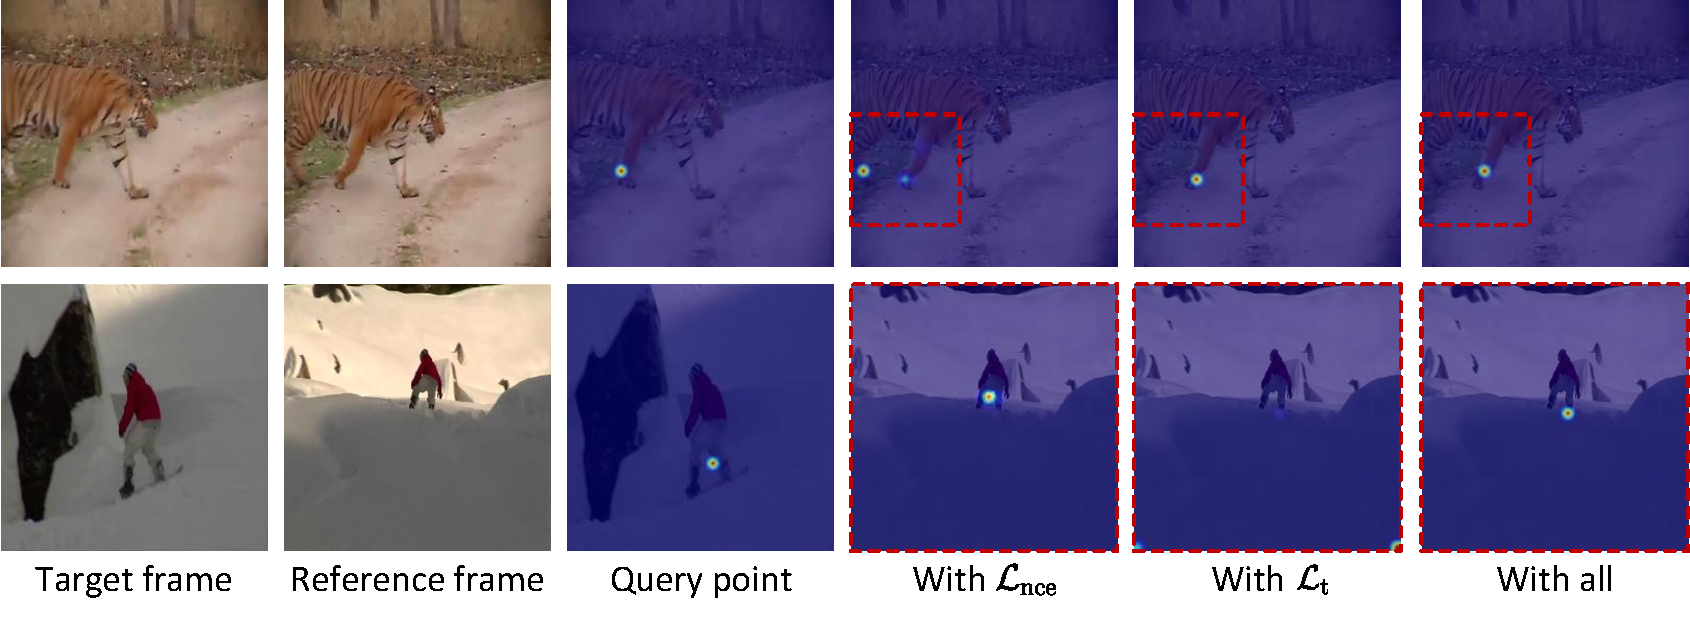
\includegraphics[width=0.8\textwidth]{figure/abalations/ablataions.pdf}}
  \caption{\small Visualization of the ablation study. Given a query point randomly sampled in target frame, we visualize the result of computing the local correlation and global correlation map $w.r.t.$ reference frame. The dashed line in red represents the range of computing correlation map $w.r.t.$ query point. The reference frame is randomly sampled in the memory bank of inference strategy [11]. }
  \label{fig:ablations}
  \vspace{-7mm}
\end{figure}


\textbf{Further analysis.} 
We give a further analysis here based on the above experiments. On the one hand, temporal feature learning helps to learn the fine-grained correspondence related to motion estimation between frames, which is unable to accomplish by training an appearance model. As you can see in the first row of Figure \ref{fig:ablations}, the appearance model trained with $\mathcal{L}_{\mathrm{nce}}$ is misled by two patches at different locations ( $i.e.$ two feats of the tiger ) which has similar appearance, while the model trained with $\mathcal{L}_{\mathrm{t}}$ tends to learn a better temporal representation for fine-grained correspondence. However, in the second row of Figure \ref{fig:ablations}, the model trained with $\mathcal{L}_{\mathrm{t}}$ fails to capture temporal correspondence with a local correlation  when facing severe temporal discontinuity  while the model trained with $\mathcal{L}_{\mathrm{nce}}$ is able to correct the mistakes by tracking the points based on the object appearance ( see with $\mathcal{L}_{\mathrm{nce}}$ and with all ).

\subsection{Comparison with State-of-the-art}
\textbf{Results for video object segmentation.}
We compare our method against previous self-supervised methods in Table \ref{table:sota}. For fair comparison, we report both results with setting the stride of encoder to 4 and 8. The results are all reported with layer $res4$ across all methods. Our method achieves state-of-the-art performance using both ResNet-18 and ResNet-50. For ResNet-18, our method with a stride of 8 achieves 70.5\%, making a absolute performance improvement by 1.2\% over all baselines using same architecture. Benefiting from less information lost for temporal feature learning by setting the stride of encoder to 4, the performance of method reaches 73.2\%, leading a performance gain of 3.5\% over MAMP, which consistently verify the idea of our methods. Besides, we found our method trained with only temporal feature learning  reaches 69.0\%/71.2\% with stride of 8/4, surpassing all methods pre-trained on Kinetics and TrackingNet which have much bigger size than YouTube-VOS. For ResNet-50, our method still outperforms all baseline methods by 2.4\%. More remarkably, our method even outperforms some task-specific fully-supervised algorithms [14][15].

\begin{table*}[t]
	\centering
	\small
	\resizebox{0.99\textwidth}{!}{
		\setlength\tabcolsep{7.3pt}
		\renewcommand\arraystretch{1.05}
		\begin{tabular}{ccccccccc}
			\toprule
      & &  & & \multicolumn{2}{c}{Dataset} & & &  \\
      \cline{5-6}
			\multirow{-2}{*}{Method} & \multirow{-2}{*}{Sup.} & \multirow{-2}{*}{Arch} & \multirow{-2}{*}{Stride} & Image & Video & \multirow{-2}{*}{$\mathcal{J}$\&$\mathcal{F}_m$ $\uparrow$} & \multirow{-2}{*}{$\mathcal{J}_m$ $\uparrow$}  &  \multirow{-2}{*}{$\mathcal{F}_m$ $\uparrow$}   \\  \hline
      Supervised &$\checkmark$ & ResNet-18 & 8 & ImageNet & -
			& 62.9 & 60.6  & 65.2  \\
      MoCo & & ResNet-18 & 8 & ImageNet &-
			& 60.8 & 58.6  & 63.1  \\
      % DetCo & ResNet-18 & 8 & I &-
			% & 61.7 & 59.6  & 62.8  \\
      SimSiam & & ResNet-18 & 8 & ImageNet &-
			& 62.0 & 60.0  & 64.0  \\
			Colorization & & ResNet-18 & 8 & - & Kinetics
			& 34.0 & 34.6  & 32.7 \\
			CorrFlow & & ResNet-18 & 8 & - & OxUvA
			& 50.3 & 48.4  & 52.2  \\
			MuG & & ResNet-18 &  8 & - & OxUvA
			& 54.3 & 52.6 & 56.1   \\
			ContrastCorr & & ResNet-18 & 8 & COCO  & TrackingNet
			& 63.0 & 60.5  & 65.5  \\
      UVC  & & ResNet-18 & 8 & COCO & Kinetics
			& 57.8 & 56.3  & 59.2  \\
			VFS  & & ResNet-18 & 8 & - & Kinetics
			& 66.7 & 64.0  & 69.4  \\
      CRW & & ResNet-18 & 8 & - & Kinetics
			& 67.6 & 64.8  & 70.2  \\
			JSTG & & ResNet-18 & 8 & - & Kinetics
			& 68.7 & 65.8   & 71.6  \\
      DUL & & ResNet-18 & 8 & - & YTV
			& 69.3 & 67.1   & 71.6  \\
      MAST & & ResNet-18 & 4 & - & YTV
			& 65.5 & 63.3  & 67.6  \\
      MAMP & & ResNet-18 & 4 & - & YTV
			& 69.7 & 68.3   & 71.2  \\
			% CLTC  & ResNet-18 & 8 & YT &(~-~, 5.58 hours)
			% & 70.3 & 67.9 & 78.2 & 72.6 & 83.7 \\
      \hline
			\textbf{Ours} & & ResNet-18 & 8 & - & YTV
			& 69.0 & & \\
      \textbf{Ours} & & ResNet-18 & 8 & ImageNet & YTV
			& 70.5   & & \\
      \textbf{Ours} & & ResNet-18 & 4 & - & YTV
			& 71.3    & & \\
      \textbf{Ours} & & ResNet-18 & 4 & ImageNet & YTV
			& \textbf{73.2}   & &  \\
			\hline
      \hline
      Supervised & $\checkmark$& ResNet-50 & 8 & ImageNet &-
			& 66.0 & 63.7  & 68.4  \\
      MoCo & & ResNet-50 & 8 & ImageNet &-
			& 65.4 & 63.2  & 67.6  \\
      SimSiam & & ResNet-50 & 8 & ImageNet &-
			& 66.3 & 64.5  & 68.2  \\
      % DetCo & ResNet-50 & 8 & I &-
			% & 66.5 & 64.7  & 68.4  \\
      TimeCycle & & ResNet-50 & 8 & - & VLOG
			& 48.7 & 46.4  & 50.0  \\
      \textcolor{red}{UVC}  & & ResNet-50 & 8 & COCO & Kinetics
			& 57.8 & 56.3  & 59.2  \\
      VINCE & & ResNet-50 & 8 & - & Kinetics
			& 65.6 & 63.4  & 67.8  \\
      SeCo & & ResNet-50 & 8 & - & Kinetics
			& 60.6 & 60.4  & 62.8  \\
      VFS  & & ResNet-50 & 8 & - & Kinetics
			& 68.9     \\
      \hline
      \textbf{Ours} & & ResNet-50 & 8 & ImageNet & YTV
			& \textbf{71.3}   & &  \\
      \hline
      \textcolor{gray}{SiamMask} & \textcolor{gray}{$\checkmark$} & \textcolor{gray}{ResNet-50} & \textcolor{gray}{-} & \textcolor{gray}{I + C} & \textcolor{gray}{YTV}
			& \textcolor{gray}{56.4} & \textcolor{gray}{54.3}  & \textcolor{gray}{58.5}  \\
      \textcolor{gray}{OnAVOS} & \textcolor{gray}{$\checkmark$} & \textcolor{gray}{ResNet-38} & \textcolor{gray}{-} & \textcolor{gray}{I + C + P} & \textcolor{gray}{D}
			& \textcolor{gray}{65.4} & \textcolor{gray}{61.6}  & \textcolor{gray}{69.1}  \\
      \textcolor{gray}{OSVOS-S}  & \textcolor{gray}{$\checkmark$} & \textcolor{gray}{VGG-16} & \textcolor{gray}{-} & \textcolor{gray}{I + P} & \textcolor{gray}{D}
			& \textcolor{gray}{68.0}   & \textcolor{gray}{64.7} & \textcolor{gray}{71.3}  \\
			\bottomrule
		\end{tabular}
	}
	\captionsetup{font=footnotesize}
	\caption{\textbf{Quantitative results for video object segmentation on validation set of DAVIS-2017}. We show results of state-of-the-art self-supervised methods and some \textcolor{gray}{supervised} methods for comparison. "Dataset" represents the dataset(s) for pre-training, including: ~I:ImageNet~(1.28m). ~C:COCO~(30k). ~O:OxUvA~(14h). ~T:TrackingNet~(300h). ~K:Kinetics~(800h). ~V:VLOG~(344h). ~YTV:YouTube-VOS~(5h). ~D:DAVIS 2017~(-). ~P:PASCAL-VOC~(-). We report the data size for self-supervised methods~(~total number/duration of image/video dataset~).}
	\label{table:sota}
	\vspace{-17pt}
\end{table*}

\begin{wraptable}{r}{8cm}
	\centering
	\small
	\resizebox{0.5\textwidth}{!}{
			\setlength\tabcolsep{3pt}
		\renewcommand\arraystretch{1.05}
		\begin{tabular}{ccccc}
            \toprule
		     & & \multicolumn{1}{c}{VIP} & \multicolumn{2}{c}{JHMDB} \\ \cline{3-5}
            \multirow{-2}{*}{Methods} & \multirow{-2}{*}{Sup.} & mIoU $\uparrow$   & PCK@0.1 $\uparrow$ & PCK@0.2 $\uparrow$
			\\ \midrule
      ResNet-18 & $\checkmark$ & 31.9 & 53.8 & 74.6 \\
      % ResNet-50 & $\checkmark$ & 39.5 & 59.2 & 78.3 \\
			TimeCycle &  & 28.9 & 57.3 & 78.1 \\
			UVC &  & 34.1  & 58.6 & 79.6\\
			CRW &  & 38.6  & 59.3 & 80.3 \\
			ContrastCorr &  & 37.4  & 61.1 & 80.8 \\
			VFS  &  & 39.9  & 60.5 & 79.5\\
			CLTC &  & 37.8  & 60.5 & 82.3\\
			JSTG &  & 40.2  & 61.4 & \textbf{85.3}\\
			\textbf{Ours} &  & \textbf{41.0} & \textbf{63.1} & 82.9\\
      \hline
      \textcolor{gray}{ATEN} & \textcolor{gray}{$\checkmark$} & \textcolor{gray}{37.9} & \textcolor{gray}{-} & \textcolor{gray}{-}\\
      \textcolor{gray}{Thin-Slicing Net} & \textcolor{gray}{$\checkmark$} & \textcolor{gray}{-} & \textcolor{gray}{68.7} & \textcolor{gray}{92.1}\\
			\bottomrule
		\end{tabular}
	}
	\captionsetup{font=small}
	\caption{\textbf{Quantitative results for human part propagation and human pose tracking.} We show results of state-of-the-art self-supervised methods and some \textcolor{gray}{supervised} methods for comparison.}
	\label{table:vip}
	\vspace{-5pt}
\end{wraptable}

\textbf{Results for human part propagation.} Next, we evaluate our method on human part tracking. Experiments are conducted on the validation set of VIP [11], which consists of 50 videos with 19 human semantic part classes, requiring more precise matching than DAVIS. Following [45], we adopt mean intersection-over-union (mIoU) as our evaluation metric and resize the video frames to 560 $\times$ 560. All models except Time-Cycle~\cite{wang2019learning} are set to ResNet-18 with a stride of 8 for fair comparison.  The results are shown in Table \ref{table:vip}. Our method achieves state-of-the-art performance, surpassing all previous state-of-the-art by 0.8\%. Notably, our model outperforms ATEN [18] which is specifically designed for the task using human annotations. Figure \ref{fig:quan} (b) depicts some visualization results on several representative videos.

  

\textbf{Results for human pose tracking.} We then make performance comparison on the downstream task of human pose tracking. We conduct the experiments on the validation of JHMDB [35] which has 268 videos.  The annotations consist of 15 body joints for each person. Probability of correct keypoint(PCK) [101] is utilized here to examine the accuracy between result and  ground-truth with different thresholds. Follow the evaluation protocol of [24, 15], we resize the video frames to 320 $\times$ 320. The results in Table \ref{table:vip} show a consistently performance gain over previous methods, which successfully demonstrates the transferability of our method to different downstream tasks. The visualization results in Figure \ref{fig:quan}~(c) show the robustness of our approach towards various challenges.


\begin{figure}[!tb]
  \centering
  {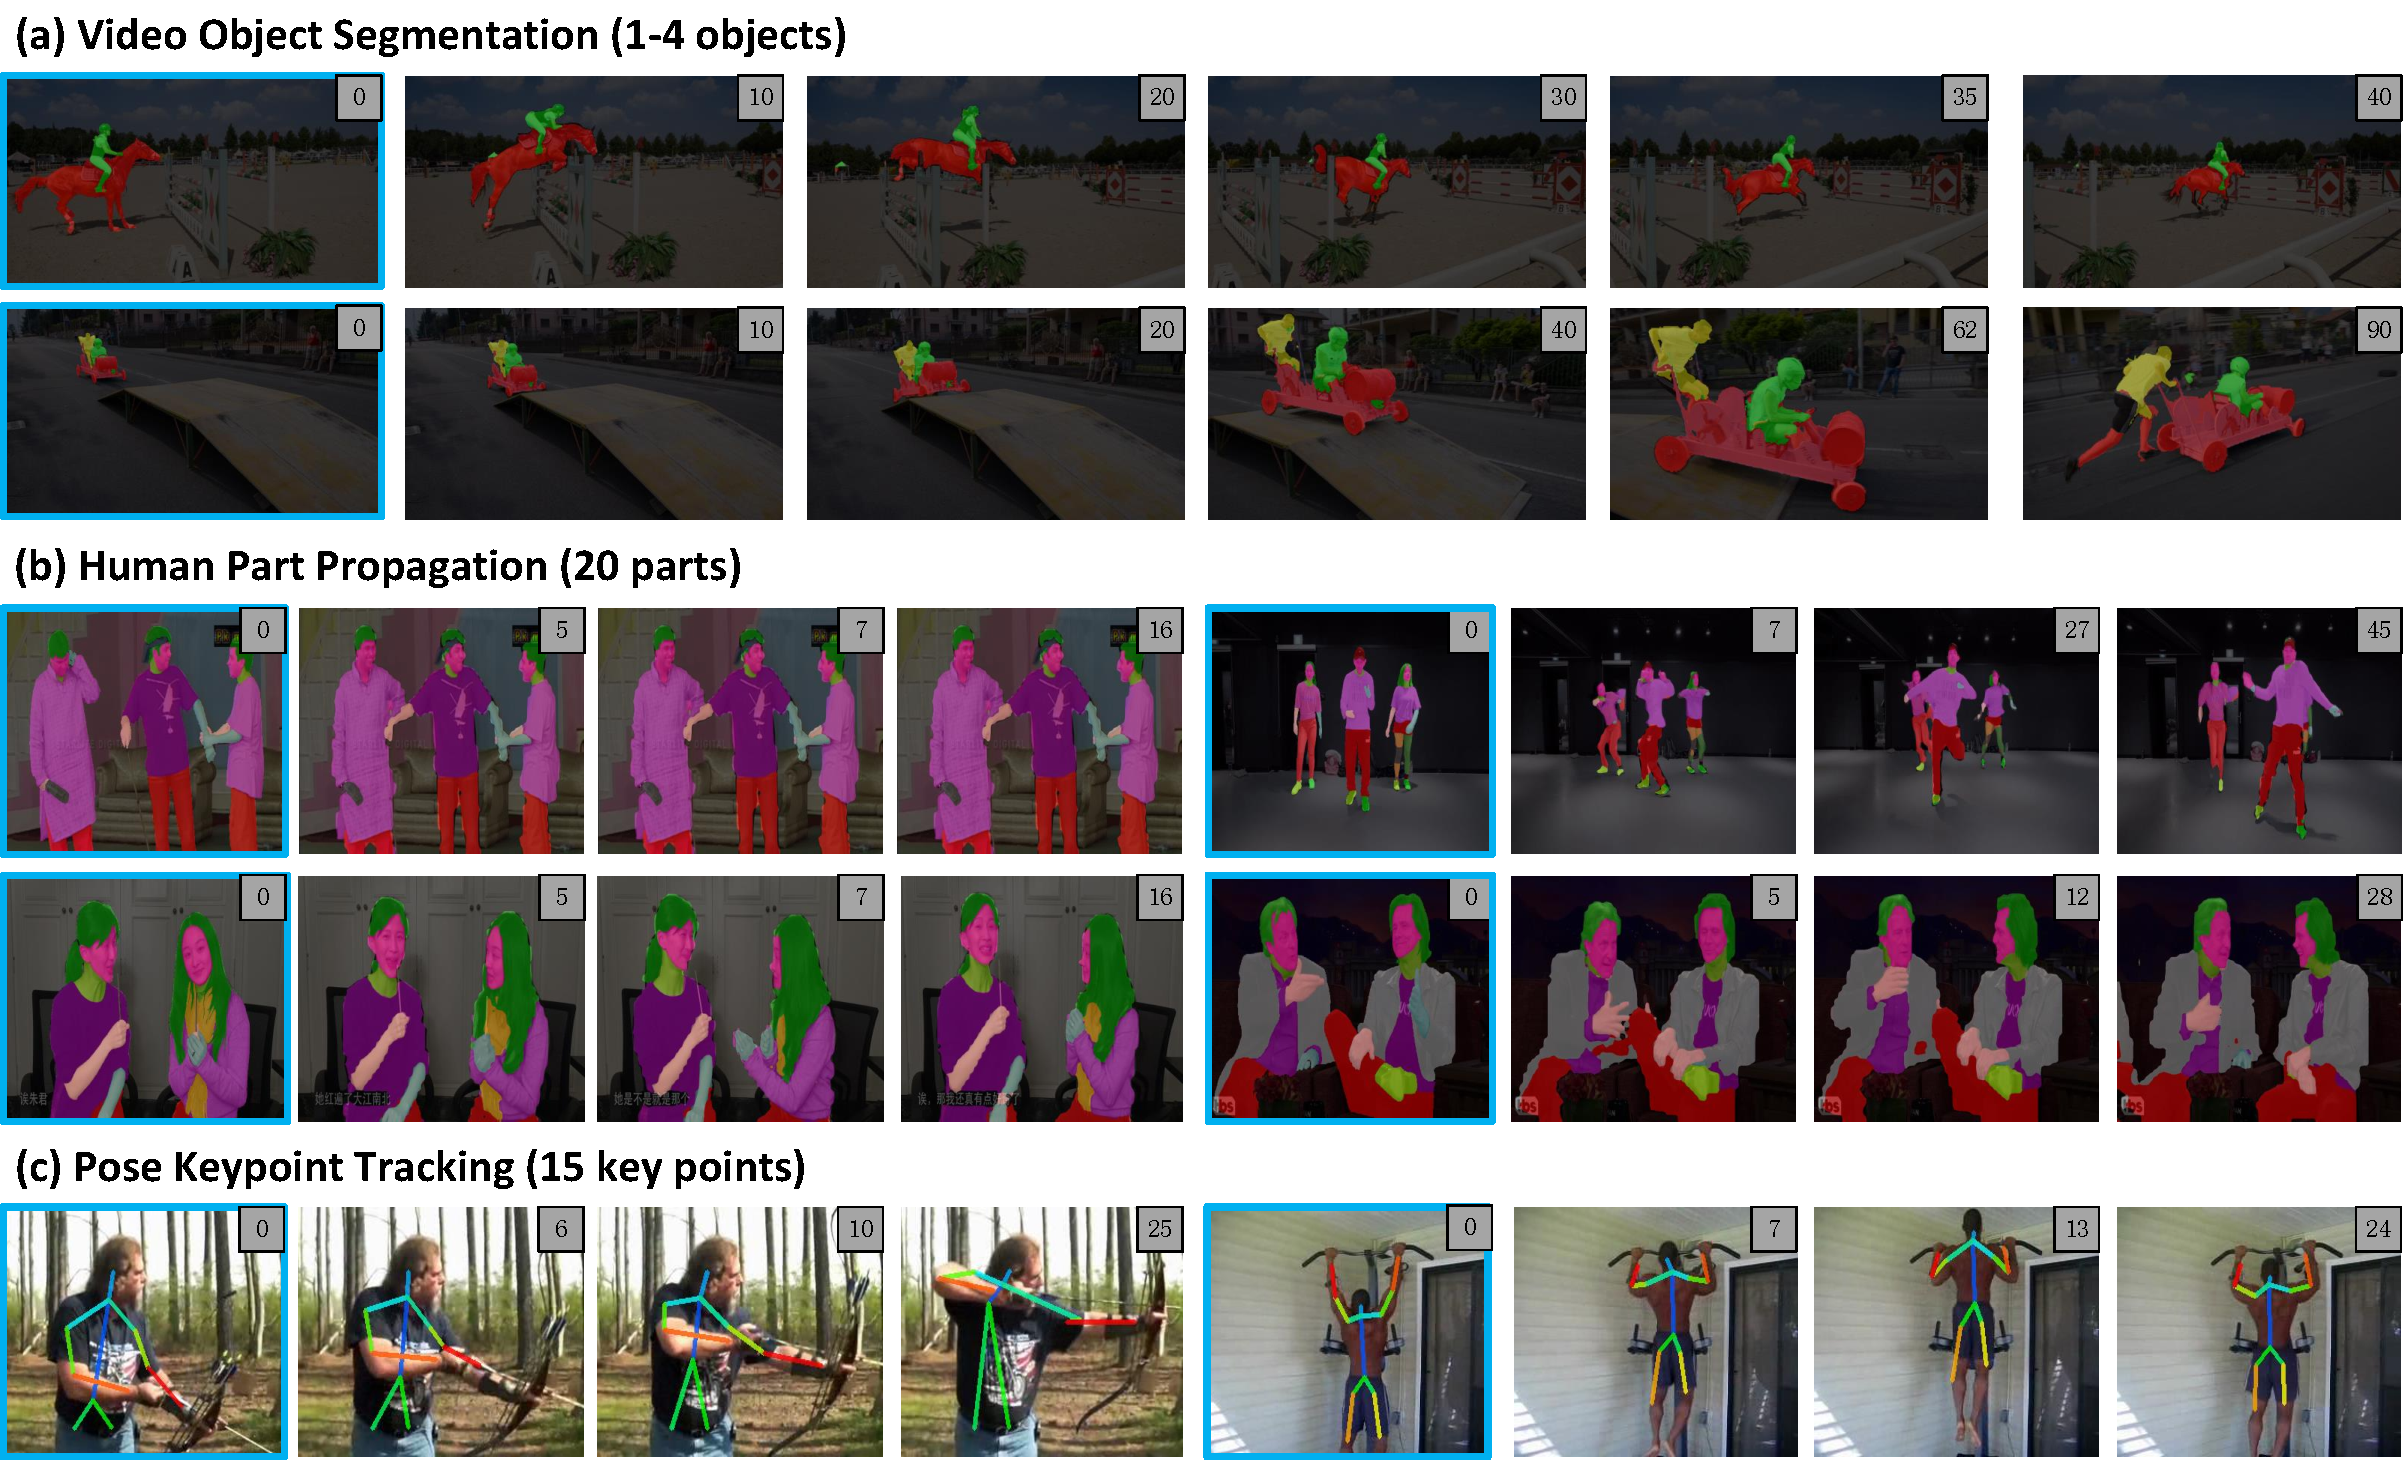
\includegraphics[width=1.0\textwidth]{figure/quantitative_results/quan.pdf}}
  \caption{\small Qualitative results for label propagation. Given a first frame with different annotation highlighted with a blue outline, we propagate it to current frame without fine-tuning. (a) Video object segmentation on DAVIS-2017. (b) Human part propagation on VIP. (c) Pose keypoint tracking on JHMDB. }
  \label{fig:quan}
  \vspace{-3mm}
\end{figure}

\section{Conclusions}
We then make performance comparison on the downstream task of human pose tracking. We conduct the experiments on the validation of JHMDB [35] which has 268 videos. The annotations consist of 15 body joints for each person. Probability of correct keypoint(PCK) [101] is utilized here to examine the accuracy between result and  ground-truth with a threshold $\sigma $. The results in Table \ref{table:vip} show a consistently performance gain over previous methods, which successfully demonstrates the transferability of our method to different downstream tasks.We then make performance comparison on the downstream task of human pose tracking. We conduct the experiments on the validation of JHMDB [35] which has 268 videos. The annotations consist of 15 body joints for each person. Probability of correct keypoint(PCK) [101] is utilized here to examine the accuracy between result and  ground-truth with different thresholds. The results in Table \ref{table:vip} show a consistently performance gain over previous methods, which successfully demonstrates the transferability of our method to different downstream tasks.


\medskip


{
\small

\bibliographystyle{abbrvnat}
\bibliography{neurips_2022}
}
% {\small
% \bibliographystyle{ieee_fullname}
% \bibliography{neurips_2022}
% }


%%%%%%%%%%%%%%%%%%%%%%%%%%%%%%%%%%%%%%%%%%%%%%%%%%%%%%%%%%%%
\section*{Checklist}


%%% BEGIN INSTRUCTIONS %%%
The checklist follows the references.  Please
read the checklist guidelines carefully for information on how to answer these
questions.  For each question, change the default \answerTODO{} to \answerYes{},
\answerNo{}, or \answerNA{}.  You are strongly encouraged to include a {\bf
justification to your answer}, either by referencing the appropriate section of
your paper or providing a brief inline description.  For example:
\begin{itemize}
  \item Did you include the license to the code and datasets? \answerYes
  \item Did you include the license to the code and datasets? \answerNo{The code and the data are proprietary.}
  \item Did you include the license to the code and datasets? \answerNA{}
\end{itemize}
Please do not modify the questions and only use the provided macros for your
answers.  Note that the Checklist section does not count towards the page
limit.  In your paper, please delete this instructions block and only keep the
Checklist section heading above along with the questions/answers below.
%%% END INSTRUCTIONS %%%


\begin{enumerate}


\item For all authors...
\begin{enumerate}
  \item Do the main claims made in the abstract and introduction accurately reflect the paper's contributions and scope?
    \answerTODO{}
  \item Did you describe the limitations of your work?
    \answerTODO{}
  \item Did you discuss any potential negative societal impacts of your work?
    \answerTODO{}
  \item Have you read the ethics review guidelines and ensured that your paper conforms to them?
    \answerTODO{}
\end{enumerate}


\item If you are including theoretical results...
\begin{enumerate}
  \item Did you state the full set of assumptions of all theoretical results?
    \answerTODO{}
        \item Did you include complete proofs of all theoretical results?
    \answerTODO{}
\end{enumerate}


\item If you ran experiments...
\begin{enumerate}
  \item Did you include the code, data, and instructions needed to reproduce the main experimental results (either in the supplemental material or as a URL)?
    \answerTODO{}
  \item Did you specify all the training details (e.g., data splits, hyperparameters, how they were chosen)?
    \answerTODO{}
        \item Did you report error bars (e.g., with respect to the random seed after running experiments multiple times)?
    \answerTODO{}
        \item Did you include the total amount of compute and the type of resources used (e.g., type of GPUs, internal cluster, or cloud provider)?
    \answerTODO{}
\end{enumerate}


\item If you are using existing assets (e.g., code, data, models) or curating/releasing new assets...
\begin{enumerate}
  \item If your work uses existing assets, did you cite the creators?
    \answerTODO{}
  \item Did you mention the license of the assets?
    \answerTODO{}
  \item Did you include any new assets either in the supplemental material or as a URL?
    \answerTODO{}
  \item Did you discuss whether and how consent was obtained from people whose data you're using/curating?
    \answerTODO{}
  \item Did you discuss whether the data you are using/curating contains personally identifiable information or offensive content?
    \answerTODO{}
\end{enumerate}


\item If you used crowdsourcing or conducted research with human subjects...
\begin{enumerate}
  \item Did you include the full text of instructions given to participants and screenshots, if applicable?
    \answerTODO{}
  \item Did you describe any potential participant risks, with links to Institutional Review Board (IRB) approvals, if applicable?
    \answerTODO{}
  \item Did you include the estimated hourly wage paid to participants and the total amount spent on participant compensation?
    \answerTODO{}
\end{enumerate}


\end{enumerate}


%%%%%%%%%%%%%%%%%%%%%%%%%%%%%%%%%%%%%%%%%%%%%%%%%%%%%%%%%%%%


\appendix


\section{Appendix}


Optionally include extra information (complete proofs, additional experiments and plots) in the appendix.
This section will often be part of the supplemental material.


\end{document}